%META {"question":"Tam giác ABC cân tại A, AH vuông góc với BC tại trung điểm H của BC. Đoạn thẳng AH là đường gì của tam giác?","options":["Đường cao (đồng thời là đường trung tuyến)","Chỉ là trung tuyến, không phải đường cao","Đường phân giác của góc B","Cạnh đáy của tam giác"],"answer":0,"note":"AH vuông góc với BC tại H nên AH là đường cao ứng với cạnh BC. Vì H là trung điểm của BC nên AH đồng thời là đường trung tuyến."}
\documentclass[border=5pt]{standalone}
\usepackage{tkz-euclide}
% Màu dùng chung cho toàn bộ hình vẽ (ảnh stack với nền tối của web)
\definecolor{tminc}{RGB}{226,232,240}   % chữ + nét chính
\definecolor{tmblue}{RGB}{0,210,255}    % nhấn neon xanh
\definecolor{tmpink}{RGB}{255,0,200}    % nhấn neon hồng
\definecolor{tmgreen}{RGB}{0,255,136}   % nhấn neon xanh lá
\color{tminc}

\begin{document}
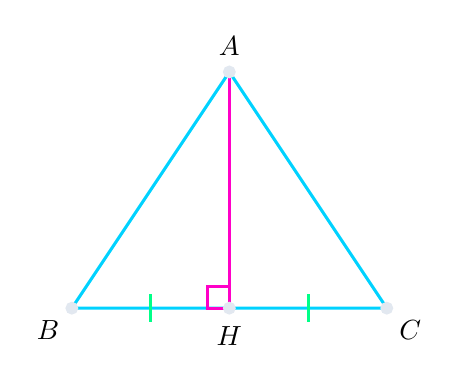
\begin{tikzpicture}[line width=1.1pt]
  \coordinate (A) at (2,3);
  \coordinate (B) at (0,0);
  \coordinate (C) at (4,0);
  \coordinate (H) at (2,0);
  \tkzDrawPolygon[tmblue,line width=1.1pt](A,B,C)
  \draw[tmpink] (A) -- (H);
  \tkzMarkRightAngles[size=0.28,color=tmpink,line width=1pt](B,H,A)
  \tkzMarkSegment[mark=|,color=tmgreen,size=5pt](B,H)
  \tkzMarkSegment[mark=|,color=tmgreen,size=5pt](H,C)
  \tkzDrawPoints[size=3.5,color=tminc,fill=tminc](A,B,C,H)
  \tkzLabelPoint[above=2pt](A){$A$}
  \tkzLabelPoint[below left=1pt](B){$B$}
  \tkzLabelPoint[below right=1pt](C){$C$}
  \tkzLabelPoint[below=3pt](H){$H$}
\end{tikzpicture}
\end{document}
